\documentclass{article}

\usepackage{arxiv}

\usepackage[utf8]{inputenc} % allow utf-8 input
\usepackage[T1]{fontenc}    % use 8-bit T1 fonts
\usepackage{lmodern}        % https://github.com/rstudio/rticles/issues/343
\usepackage{hyperref}       % hyperlinks
\usepackage{url}            % simple URL typesetting
\usepackage{booktabs}       % professional-quality tables
\usepackage{amsfonts}       % blackboard math symbols
\usepackage{nicefrac}       % compact symbols for 1/2, etc.
\usepackage{microtype}      % microtypography
\usepackage{graphicx}

\title{Unveiling Color Dynamics in Andy Warhol's ``Shot Marilyns'': A
Study on Visual Variations and Perception}

\author{
    Erick S. Arenas V
   \\
    Department of Statistics \\
    University of California, Davis \\
  Davis, CA 95616 \\
  \texttt{\href{mailto:esarenas@ucdavis.edu}{\nolinkurl{esarenas@ucdavis.edu}}} \\
   \And
    Weilin Cheng
   \\
    Department of Statistics \\
    University of California, Davis \\
  Davis, CA 95616 \\
  \texttt{\href{mailto:wncheng@ucdavis.edu}{\nolinkurl{wncheng@ucdavis.edu}}} \\
   \And
    Hengyuan Liu
   \\
    Department of Statistics \\
    University of California, Los Angeles \\
  Los Angeles, CA 90095 \\
  \texttt{\href{mailto:hengyuanliu@g.ucla.edu}{\nolinkurl{hengyuanliu@g.ucla.edu}}} \\
   \And
    Xinhui Luo
   \\
    Department of Statistics \\
    University of California, Davis \\
  Davis, CA 95616 \\
  \texttt{\href{mailto:xinluo@ucdavis.edu}{\nolinkurl{xinluo@ucdavis.edu}}} \\
   \And
    Kathy Mo
   \\
    Department of Statistics \\
    University of California, Los Angeles \\
  Los Angeles, CA 90095 \\
  \texttt{\href{mailto:kamo@ucdavis.edu}{\nolinkurl{kamo@ucdavis.edu}}} \\
   \And
    Li Yuan
   \\
    Department of Statistics \\
    University of Michigan, Ann Arbor \\
  Ann Arbor, MI 48104 \\
  \texttt{\href{mailto:leeyuan@umich.edu}{\nolinkurl{leeyuan@umich.edu}}} \\
  }


% tightlist command for lists without linebreak
\providecommand{\tightlist}{%
  \setlength{\itemsep}{0pt}\setlength{\parskip}{0pt}}



\usepackage{amsmath}
\usepackage{graphicx}
\usepackage{subcaption}
\begin{document}
\maketitle


\begin{abstract}
This study delves into the comparative analysis of five distinct
versions of Andy Warhol's ``Shot Marilyns,'' focusing on the intricacies
of their color composition and distribution. Employing a range of
analytical methods, including relative conditional entropy, this
research investigates the unique color distributions and interrelations
present in each artwork. Through the clustering of the artworks and the
meticulous examination of specified regions of interest (ROIs)---namely,
the backgrounds, hair, eyeshadow, and faces---we have unearthed profound
insights into the constructional variances and similarities among the
images. Our findings reveal that the presupposed uniformity in the
coloration of certain elements stands contradicted, thereby underscoring
the complexity and illusionary nature of color perception in visual art.
\end{abstract}

\keywords{
    shot marilyns
   \and
    marilyn monroe
   \and
    andy warhol
   \and
    region of interest
   \and
    python
  }

\hypertarget{introduction}{%
\section{Introduction}\label{introduction}}

``Shot Marilyns,'' an illustrious artwork by the American artist Andy
Warhol, stands as a testament to his exploration of celebrity culture
and the commodification of images. Created in 1964, this series features
multiple depictions of Marilyn Monroe, crafted in the wake of her
untimely demise, thereby immortalizing her status as a cultural icon.
Warhol's fascination with fame, consumerism, and the media's influence
on societal perceptions is evident in his innovative use of silkscreen
printing. This technique, adopted in August 1962, facilitated a
production-line approach in art-making, enabling Warhol to replicate
images with minor variations. The ``Shot Marilyns'' series, inspired by
Monroe's death in the same year, utilized this method to produce
screenprints of her image, employing photo stencils and a palette of
vibrant inks to transfer her likeness onto canvas. This body of work
underscores Warhol's endeavor to dissect Monroe's persona through
repetitive imagery, each variation rendered in distinct colors and
compositions, allowing for diverse visual interpretations.

The series' repetitive nature serves as a critique of the pervasive
commodification of celebrities, transforming them into ubiquitous
symbols within popular culture. Warhol's strategic use of bright,
contrasting colors aims to encapsulate Monroe's dynamic celebrity
essence, with the vivid hues underscoring her societal allure and
influence. This study seeks to analyze the pixel color distribution in
RGB space across the five ``Shot Marilyns'' images, examining the
interplay between primary colors through relative conditional entropy.
Such an analysis aims to reveal the underlying emotional and symbolic
connotations Warhol might have intended, with color distributions
potentially reflecting varied moods and themes.

In 1964, an intriguing incident further contributed to the series' lore
when Dorothy Podber, a performance artist, mistakenly received
permission from Warhol to ``shoot'' the Marilyns, leading to an act of
literal gunfire that damaged four of the five canvases. This event
birthed the ``Shot Marilyns,'' adding a layer of physical and conceptual
depth to the artwork. Part of our project involves digitally restoring
the ``Blue Marilyn,'' focusing on the gunshot damage, by analyzing and
replicating the surrounding area's color distribution.

This paper is intended for publication in the Journal on Computing and
Cultural Heritage and aims to shed light on the technological
intersections of art restoration and analysis, using Warhol's ``Shot
Marilyns'' as a pivotal study case.

\begin{figure}[ht]
  \centering
  \begin{subfigure}{0.3\textwidth}
    \centering
    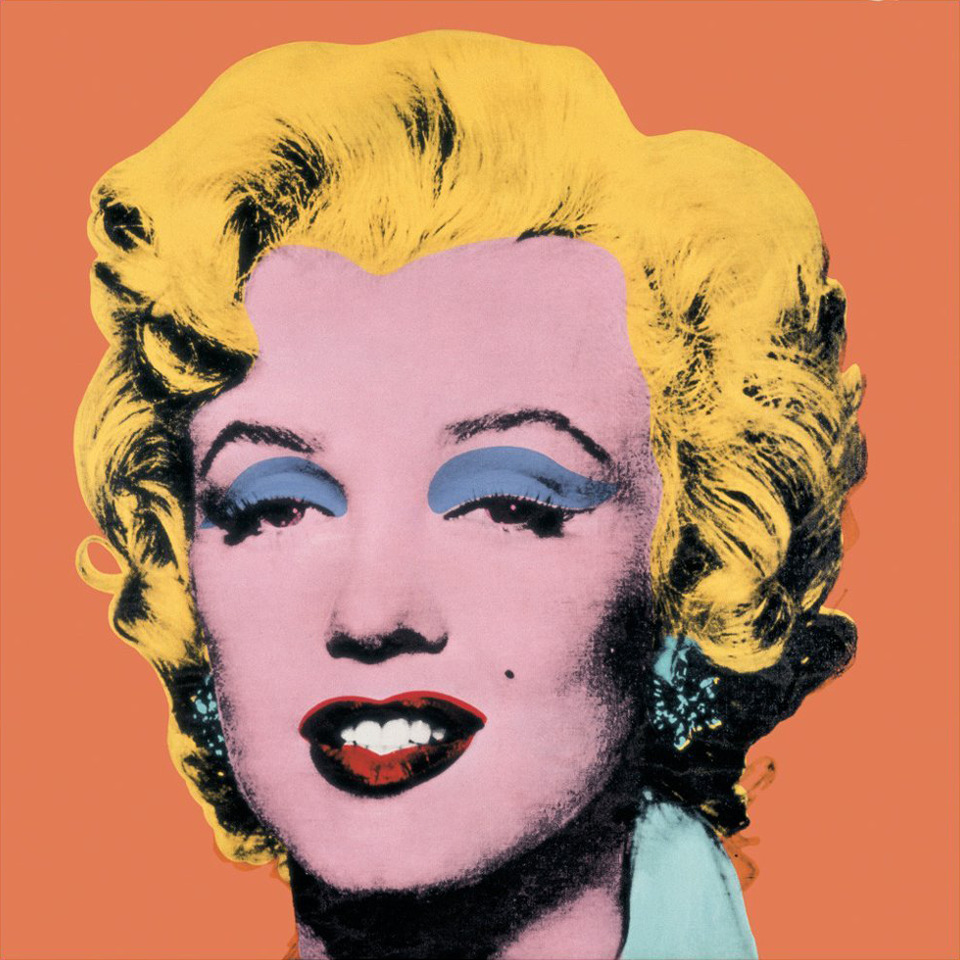
\includegraphics[width=125px]{main_files/figure-latex/1_1_orange_marilyn.jpg}
    \caption{Figure 1.1: Orange Marilyn}
    \label{fig:1_1_orange_marilyn}
  \end{subfigure}
  \hfill
  \begin{subfigure}{0.3\textwidth}
    \centering
    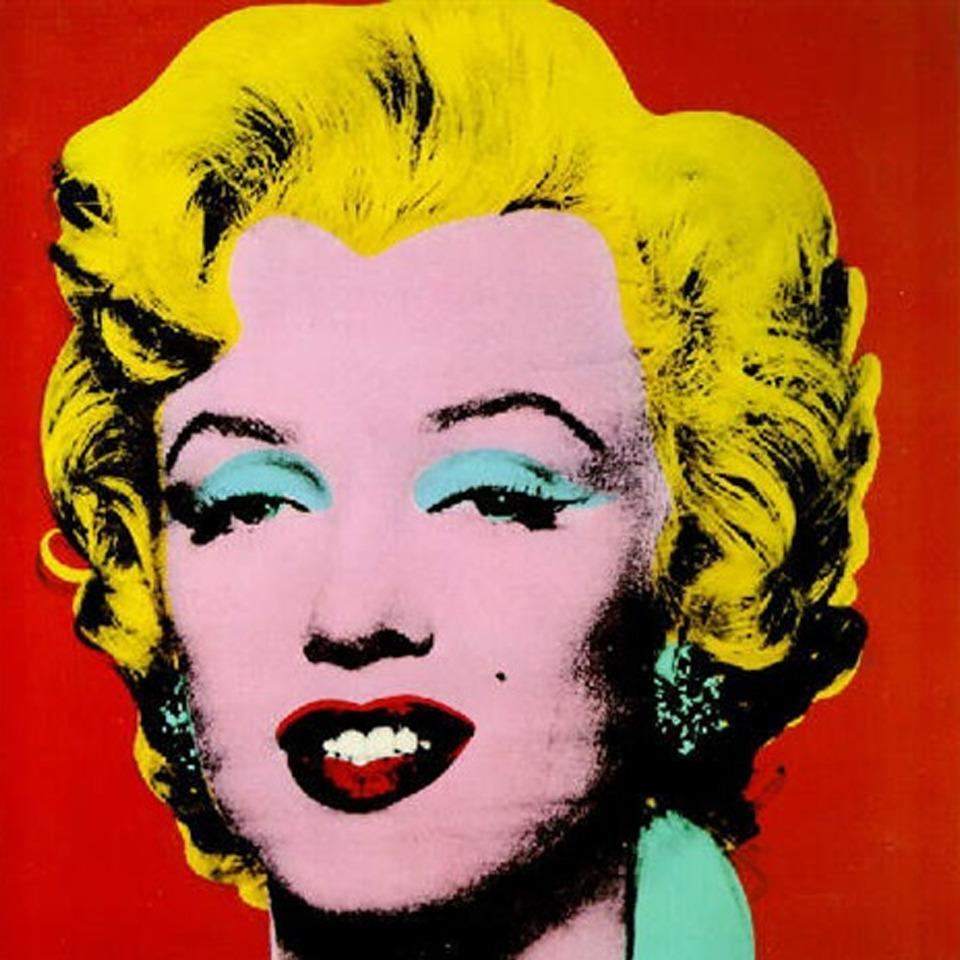
\includegraphics[width=125px]{main_files/figure-latex/1_2_red_marilyn.jpg}
    \caption{Figure 1.2: Red Marilyn}
    \label{fig:1_2_red_marilyn}
  \end{subfigure}
  \hfill
  \begin{subfigure}{0.3\textwidth}
    \centering
    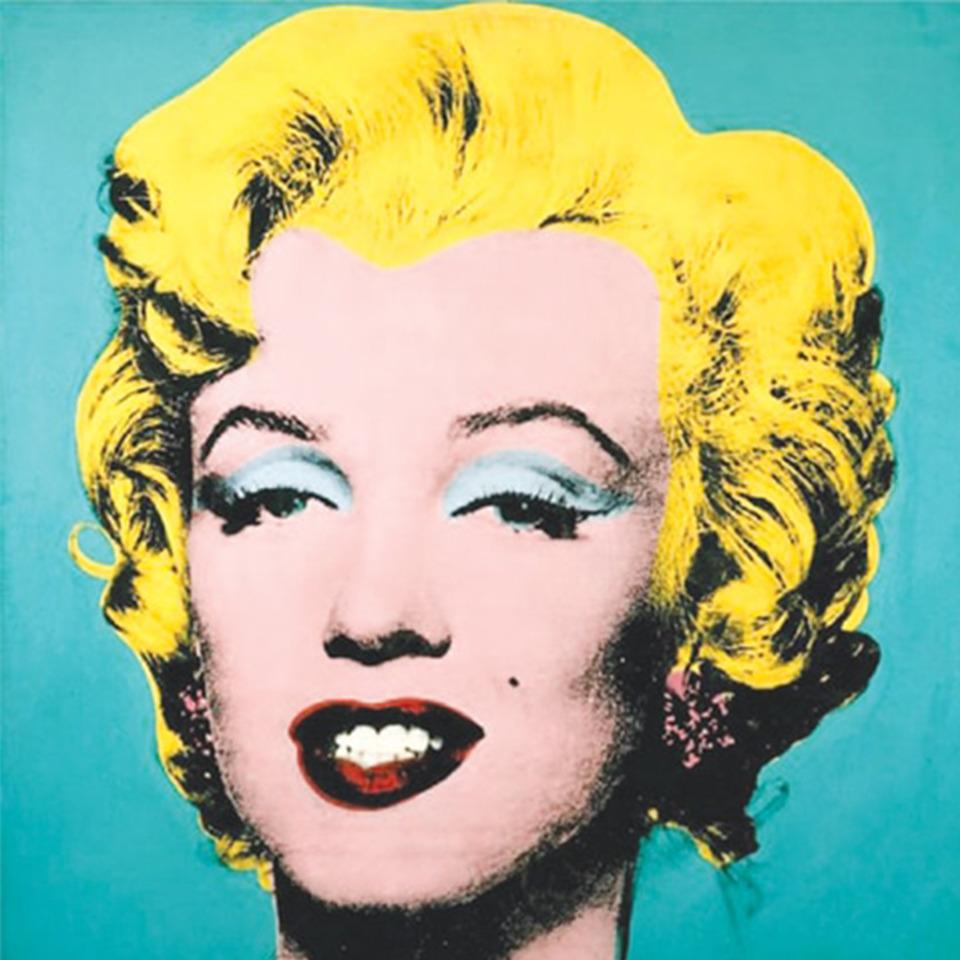
\includegraphics[width=125px]{main_files/figure-latex/1_3_turq_marilyn.jpg}
    \caption{Figure 1.3: Turquoise Marilyn}
    \label{fig:1_3_turq_marilyn}
  \end{subfigure}

  \vspace{1em} % Add some vertical space between rows

  \begin{minipage}{0.6\textwidth}
    \centering
    \begin{subfigure}{0.45\textwidth}
      \centering
      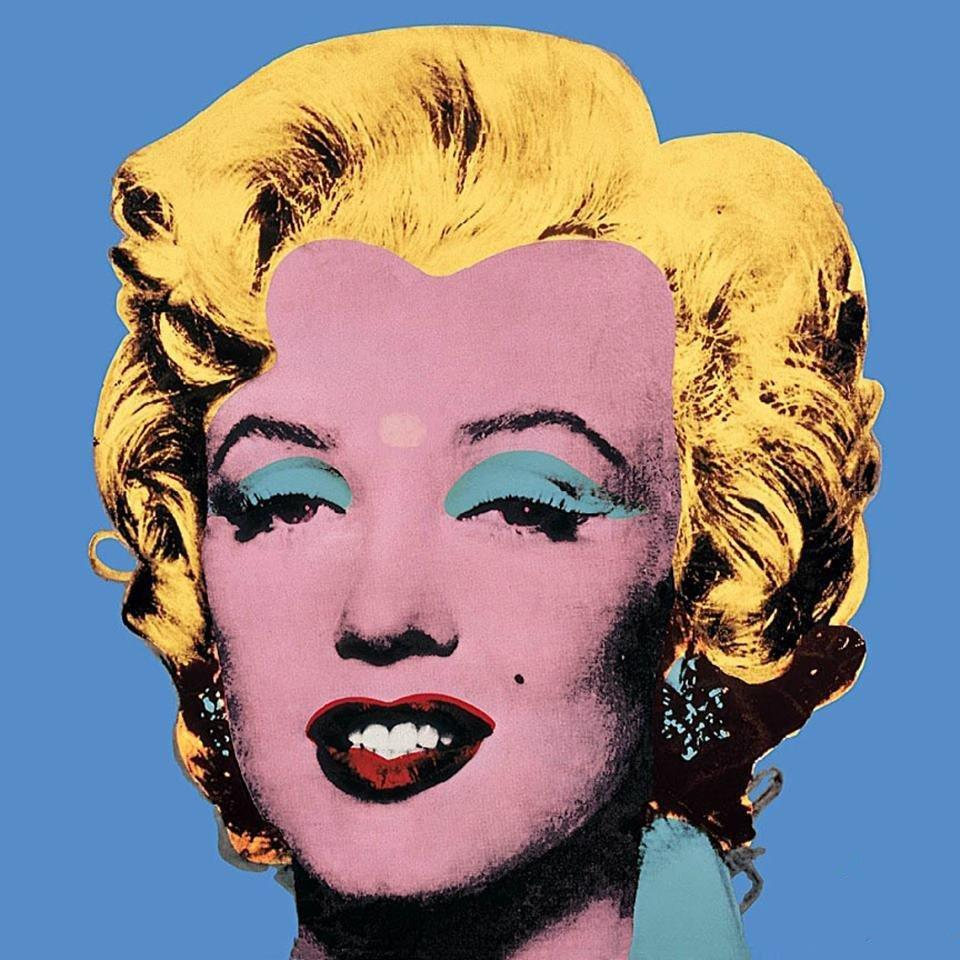
\includegraphics[width=125px]{main_files/figure-latex/1_4_blue_marilyn.jpg}
      \caption{Figure 1.4: Blue Marilyn}
      \label{fig:1_4_blue_marilyn}
    \end{subfigure}
    \hfill
    \begin{subfigure}{0.45\textwidth}
      \centering
      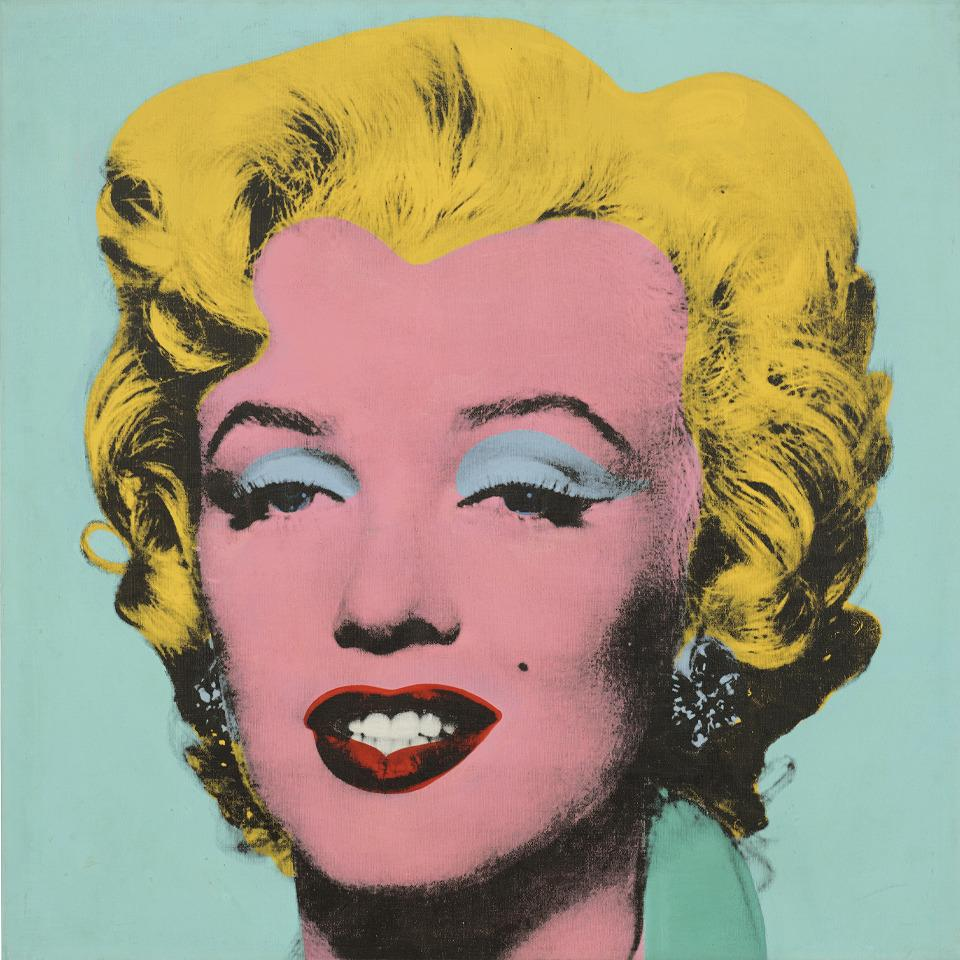
\includegraphics[width=125px]{main_files/figure-latex/1_5_eggblue_marilyn.jpg}
      \caption{Figure 1.5: Eggblue Marilyn}
      \label{fig:1_5_eggblue_marilyn}
    \end{subfigure}
  \end{minipage}

  \caption{Different color variations of Marilyn Monroe}
  \label{fig:marilyn_variations}
\end{figure}

\hypertarget{methods}{%
\section{Methods}\label{methods}}

\hypertarget{data-description}{%
\section{Data Description}\label{data-description}}

\hypertarget{data-exploration-and-visualization-analysis}{%
\section{Data Exploration and Visualization
Analysis}\label{data-exploration-and-visualization-analysis}}

\hypertarget{clustering-based-on-whole-images}{%
\section{Clustering based on Whole
Images}\label{clustering-based-on-whole-images}}

\hypertarget{clustering-based-on-region-of-interest-roi}{%
\section{Clustering based on Region of Interest
(ROI)}\label{clustering-based-on-region-of-interest-roi}}

\hypertarget{repair-gunshot-of-image}{%
\section{Repair Gunshot of Image}\label{repair-gunshot-of-image}}

\hypertarget{disuccsion}{%
\section{Disuccsion}\label{disuccsion}}

\hypertarget{conclusion-and-future-work}{%
\section{Conclusion and Future Work}\label{conclusion-and-future-work}}

\bibliographystyle{unsrt}
\bibliography{references.bib}


\end{document}
